\documentclass[11pt,letterpaper]{article}
\usepackage[utf8]{inputenc}
\usepackage[T1]{fontenc}
\usepackage[provide=*,english]{babel}
\usepackage{lmodern}
\usepackage{amsmath,amssymb,amsfonts}
\usepackage[margin=2.5cm]{geometry}
\usepackage{fancyhdr}
\usepackage{enumitem}
\usepackage[most]{tcolorbox}
\usepackage{xcolor}
\usepackage{tikz}
\usetikzlibrary{arrows.meta,angles,quotes,calc,babel}
\usepackage{placeins}
\usepackage{graphicx}
\usepackage{microtype}
\usepackage{needspace}

% ============ PALETTE: BLACK, ORANGE, AND CREAM ============
\definecolor{blackmain}{HTML}{1A1A1A}
\definecolor{orangeacc}{HTML}{E65C00}
\definecolor{creambg}{HTML}{FBF8F1}
\definecolor{orangebg}{HTML}{FFF4EB}
\definecolor{graymuted}{HTML}{7A746E}
\definecolor{pureblack}{HTML}{0D0D0D}

% ============ HEADERS AND FOOTERS ============
\setlength{\headheight}{24pt}
\pagestyle{fancy}
\fancyhf{}
\fancyhead[L]{\textcolor{blackmain}{\textbf{\small Mathematical Methods I}}}
\fancyhead[R]{\textcolor{orangeacc}{\textbf{\small Exterior derivative}}}
\fancyfoot[C]{\textcolor{graymuted}{\thepage}}
\renewcommand{\headrulewidth}{0.8pt}
\renewcommand{\headrule}{\hbox to\headwidth{\color{orangeacc}\leaders\hrule height \headrulewidth\hfill}}

\setlist[itemize]{label={\small\textcolor{orangeacc}{$\blacksquare$}},leftmargin=1.6em}
\setlist[enumerate]{label={\textcolor{orangeacc}{\arabic*.}},leftmargin=1.8em}

% ============ TITLES ============
\newcommand{\manualsection}[1]{%
  \Needspace{16\baselineskip}%
  \vspace{0.35cm}
  \par\noindent{\Large\bfseries\color{blackmain} #1}\par\nobreak
  \noindent{\color{orangeacc}\rule{\linewidth}{1.4pt}}\par\nobreak
  \vspace{0.15cm}
}

\newcommand{\manualsubsection}[1]{%
  \par\vspace{0.2cm}\noindent{\bfseries\color{orangeacc} #1}\par\nobreak
  \vspace{0.12cm}
}

% ============ CONTENT BOXES ============
\newtcolorbox{infobox}[2][orangeacc]{
  enhanced,
  colback=creambg,colframe=#1!90!black,
  boxrule=1pt,arc=2mm,
  left=9pt,right=9pt,top=5pt,bottom=5pt,
  before skip=7pt,after skip=7pt,
  before upper={\textbf{\color{#1!95!black}\large #2}\par\nobreak
    {\color{#1!50}\rule{\linewidth}{0.6pt}}\par\nobreak\smallskip}
}

\newtcolorbox{examplebox}[1]{
  enhanced,
  colback=orangebg,colframe=orangeacc!85!black,
  boxrule=1pt,arc=2mm,
  left=9pt,right=9pt,top=5pt,bottom=5pt,
  before skip=7pt,after skip=7pt,
  before upper={\textbf{\color{orangeacc!95!black}\large #1}\par\nobreak
    {\color{orangeacc!40}\rule{\linewidth}{0.6pt}}\par\nobreak\smallskip}
}

\newtcolorbox{theorembox}[1]{
  enhanced,
  colback=creambg!70!white,colframe=pureblack,
  boxrule=1.1pt,arc=2mm,
  left=9pt,right=9pt,top=5pt,bottom=5pt,
  before skip=7pt,after skip=7pt,
  before upper={\textbf{\color{pureblack}\large #1}\par\nobreak
    {\color{orangeacc}\rule{\linewidth}{0.8pt}}\par\nobreak\smallskip}
}

\newcommand{\term}[1]{\textbf{\color{orangeacc}#1}}
\newcommand{\termb}[1]{\textbf{\color{blackmain}#1}}
\renewcommand{\familydefault}{\rmdefault}
\tikzset{every node/.append style={font=\rmfamily}}

\begin{document}
\setlength{\abovedisplayskip}{6pt}
\setlength{\belowdisplayskip}{6pt}
\setlength{\abovedisplayshortskip}{4pt}
\setlength{\belowdisplayshortskip}{4pt}
\setlength{\textfloatsep}{10pt}
\setlength{\intextsep}{8pt}
\setlength{\jot}{2pt}
\color{blackmain}
\begin{center}
{\LARGE\textbf{Mathematical Methods I}}\\[0.2cm]
{\Large\textcolor{orangeacc}{\textbf{Differential forms and the exterior derivative}}}\\[0.4cm]
{\large\textcolor{graymuted}{Gabriel Velázquez}}\\[0.25cm]
\end{center}
\manualsection{1. Differential forms and degree}
Differential forms can be evaluated on vectors, pairs of vectors, and, more generally, collections of tangent vectors, while keeping track of orientation. In these notes, we work with smooth forms on an open set $\Omega\subseteq\mathbb{R}^n$.
\begin{infobox}[orangeacc]{Definition 1.1 (Differential $k$-form)}
For $k\geq1$, a $k$-form $\omega$ assigns to each point $p$ an alternating multilinear map
\[
\omega_p:\underbrace{T_p\Omega\times\cdots\times T_p\Omega}_{k\text{ factors}}\longrightarrow\mathbb{R}.
\]
Multilinearity means linearity in each argument. Alternation means that interchanging two vectors changes the sign and that the value is zero whenever two arguments coincide. A \term{0-form} is a smooth scalar function.
\end{infobox}
\manualsubsection{Degrees in $\mathbb{R}^3$}
\begin{align*}
\text{0-form:}\quad &f(x,y,z),\\
\text{1-form:}\quad &A_x\,dx+A_y\,dy+A_z\,dz,\\
\text{2-form:}\quad &F_x\,dy\wedge dz+F_y\,dz\wedge dx+F_z\,dx\wedge dy,\\
\text{3-form:}\quad &K\,dx\wedge dy\wedge dz.
\end{align*}
The coefficients are functions of the point. The 1-forms serve as line integrands, the 2-forms as oriented surface integrands, and the 3-forms as oriented volume integrands.
\begin{theorembox}{General coordinate expression}
A $k$-form can be written uniquely as
\[
\omega=\sum_{i_1<\cdots<i_k}a_{i_1\cdots i_k}(x)\,
 dx^{i_1}\wedge\cdots\wedge dx^{i_k}.
\]
The sum uses only strictly increasing indices. In dimension $n$, this basis has $\binom{n}{k}$ elements, and every form of degree $k>n$ is zero.
\end{theorembox}
In the abbreviated notation $\omega=\sum_I a_I dx^I$, the multi-index $I=(i_1,\ldots,i_k)$ is ordered and $dx^I=dx^{i_1}\wedge\cdots\wedge dx^{i_k}$.

\newpage
\manualsection{2. Wedge product and orientation}
The \term{wedge product} $\wedge$ combines a $k$-form and an $\ell$-form to produce a $(k+\ell)$-form. It is bilinear, associative, and satisfies
\[
\omega\wedge\eta=(-1)^{k\ell}\eta\wedge\omega.
\]
For 1-forms $\alpha,\beta$, this gives $\alpha\wedge\beta=-\beta\wedge\alpha$ and $\alpha\wedge\alpha=0$. In particular, $dx\wedge dx=0$: any product of coordinate differentials containing a repeated factor vanishes.
\begin{infobox}[orangeacc]{Evaluation of two 1-forms}
For vectors $u,v$ based at the same point,
\[
(\alpha\wedge\beta)(u,v)=\alpha(u)\beta(v)-\alpha(v)\beta(u).
\]
Thus, $(dx\wedge dy)(u,v)=u^xv^y-u^yv^x$ is the signed area of the projections of $u,v$ onto the $xy$-plane.
\end{infobox}
\begin{figure}[htbp]
\centering
\begin{tikzpicture}[>=Stealth,scale=.78]
\coordinate (O) at (0,0); \coordinate (U) at (3,0); \coordinate (V) at (1,2);
\fill[orangebg] (O)--(U)--(4,2)--(V)--cycle;
\draw[graymuted,dashed] (U)--(4,2)--(V);
\draw[->,orangeacc,very thick] (O)--(U) node[midway,below] {$u=(3,0)$};
\draw[->,blackmain,very thick] (O)--(V) node[midway,left] {$v=(1,2)$};
\draw[->,orangeacc] (.65,0) arc (0:63.435:.65);
\node at (2.35,1.1) {$+6$};
\node[anchor=west,align=left] at (5,1.2) {$(dx\wedge dy)(u,v)=6$\\[6pt]$(dx\wedge dy)(v,u)=-6$};
\end{tikzpicture}
\caption{The order $(u,v)$ gives the positive orientation. Interchanging the vectors preserves the geometric area and changes its sign.}
\end{figure}
\FloatBarrier
\begin{theorembox}{Oriented volume}
The Euclidean volume form satisfies
\[
(dx\wedge dy\wedge dz)(u,v,w)
=\det\begin{pmatrix}u^x&v^x&w^x\\u^y&v^y&w^y\\u^z&v^z&w^z\end{pmatrix}.
\]
Its absolute value is the volume of the parallelepiped spanned by the three vectors; the sign records its orientation.
\end{theorembox}
\begin{figure}[htbp]
\centering
\begin{tikzpicture}[>=Stealth,scale=.72]
\coordinate (O) at (0,0); \coordinate (U) at (3,0); \coordinate (V) at (1,1); \coordinate (W) at (.3,2);
\fill[orangebg] (O)--(U)--(3.3,2)--(W)--cycle;
\draw[graymuted,dashed] (V)--(4,1) (V)--(1.3,3);
\draw[graymuted] (U)--(4,1)--(4.3,3)--(3.3,2)--cycle;
\draw[graymuted] (W)--(1.3,3)--(4.3,3) (W)--(3.3,2);
\draw[->,orangeacc,very thick] (O)--(U) node[midway,below] {$u$};
\draw[->,blackmain,very thick] (O)--(V) node[midway,right=5pt] {$v$};
\draw[->,blackmain,very thick] (O)--(W) node[midway,left=5pt] {$w$};
\end{tikzpicture}
\caption{Projection of a parallelepiped. The determinant is calculated using the vectors in space, not their projections in the drawing.}
\end{figure}
\FloatBarrier

\newpage
\manualsection{3. Wedge product and Jacobian}
Let $x=x(u,v)$, $y=y(u,v)$ be a locally invertible change of coordinates. By the chain rule,
\[
dx=x_u\,du+x_v\,dv,\qquad dy=y_u\,du+y_v\,dv,
\]
where $x_u=\partial x/\partial u$, and similarly for the other coefficients.
\manualsubsection{Expansion in two dimensions}
We expand without changing the order of the differentials:
\begin{align*}
dx\wedge dy
&=(x_u\,du+x_v\,dv)\wedge(y_u\,du+y_v\,dv)\\
&=x_uy_u\,du\wedge du+x_uy_v\,du\wedge dv\\
&\quad+x_vy_u\,dv\wedge du+x_vy_v\,dv\wedge dv.
\end{align*}
The repeated terms vanish and $dv\wedge du=-du\wedge dv$. Therefore,
\begin{theorembox}{Theorem 3.1 (Transformation of the oriented area element)}
\[
\boxed{dx\wedge dy=(x_uy_v-x_vy_u)\,du\wedge dv
=\det(J)\,du\wedge dv,}
\qquad
J=\begin{pmatrix}x_u&x_v\\y_u&y_v\end{pmatrix}.
\]
The determinant appears because the wedge product is alternating.
\end{theorembox}
\begin{examplebox}{Example 3.2 (Polar coordinates)}
With $x=r\cos\theta$, $y=r\sin\theta$, $r>0$, and a local choice of angle,
\[
dx=\cos\theta\,dr-r\sin\theta\,d\theta,
\qquad dy=\sin\theta\,dr+r\cos\theta\,d\theta.
\]
Expanding and eliminating the repeated terms,
\begin{align*}
dx\wedge dy
&=r\cos^2\theta\,dr\wedge d\theta
-r\sin^2\theta\,d\theta\wedge dr\\
&=r(\cos^2\theta+\sin^2\theta)\,dr\wedge d\theta\\
&=r\,dr\wedge d\theta.
\end{align*}
The sign of the second term changes when $d\theta\wedge dr$ is reordered.
\end{examplebox}
\begin{infobox}[blackmain]{Determinant and absolute value}
Forms record orientation and transform by $\det J$. When changing variables in an integral with respect to unoriented area or volume, $|\det J|$ appears instead. For example, interchanging $u$ and $v$ changes the sign of $du\wedge dv$.
\end{infobox}

\newpage
\manualsection{4. The Jacobian in dimension $n$}
Let $x^1,\ldots,x^n$ be functions of new coordinates $u^1,\ldots,u^n$, with invertible Jacobian
\[
J^i{}_j=\frac{\partial x^i}{\partial u^j},
\qquad dx^i=\sum_{j=1}^n J^i{}_j\,du^j.
\]
\begin{theorembox}{Theorem 4.1 (Transformation of a top-degree form)}
\[
\boxed{dx^1\wedge\cdots\wedge dx^n
=\det(J)\,du^1\wedge\cdots\wedge du^n.}
\]
\end{theorembox}
\manualsubsection{Proof using the Levi-Civita symbol}
The completely antisymmetric symbol $\varepsilon_{j_1\cdots j_n}$ is defined by
\[
\varepsilon_{j_1\cdots j_n}=\begin{cases}
+1,&(j_1,\ldots,j_n)\text{ is an even permutation of }(1,\ldots,n),\\
-1,&(j_1,\ldots,j_n)\text{ is an odd permutation},\\
0,&\text{there are repeated indices}.
\end{cases}
\]
The alternating property of the wedge product is then expressed as
\[
du^{j_1}\wedge\cdots\wedge du^{j_n}
=\varepsilon_{j_1\cdots j_n}\,du^1\wedge\cdots\wedge du^n.
\]
Substituting $dx^i=\sum_{j_i=1}^n J^i{}_{j_i}du^{j_i}$ and expanding,
\begin{align*}
dx^1\wedge\cdots\wedge dx^n
&=\sum_{j_1,\ldots,j_n=1}^n
J^1{}_{j_1}\cdots J^n{}_{j_n}\,
 du^{j_1}\wedge\cdots\wedge du^{j_n}\\
&=\left(\sum_{j_1,\ldots,j_n=1}^n
\varepsilon_{j_1\cdots j_n}J^1{}_{j_1}\cdots J^n{}_{j_n}\right)
 du^1\wedge\cdots\wedge du^n.
\end{align*}
Terms with repeated indices vanish. The remaining terms correspond to permutations $\sigma\in S_n$, so the coefficient is
\[
\sum_{\sigma\in S_n}\varepsilon_{\sigma(1)\cdots\sigma(n)}
\frac{\partial x^1}{\partial u^{\sigma(1)}}\cdots
\frac{\partial x^n}{\partial u^{\sigma(n)}}
=\det\left(\frac{\partial x^i}{\partial u^j}\right).
\]
Substituting this determinant into the preceding expansion proves the theorem.
\begin{examplebox}{Example 4.2 (Cylindrical coordinates)}
For $x=r\cos\theta$, $y=r\sin\theta$, $z=z$, with $r>0$, the Jacobian has the polar block and a $1$ in the $z$ direction. Thus, $\det J=r$ and
\[
dx\wedge dy\wedge dz=r\,dr\wedge d\theta\wedge dz.
\]
\end{examplebox}

\newpage
\manualsection{5. The exterior derivative}
\begin{infobox}[orangeacc]{Definition 5.1 (The operator $d$)}
The \term{exterior derivative} raises the degree of a form by one:
\[
d:\Omega^k(\Omega)\longrightarrow\Omega^{k+1}(\Omega).
\]
Here $\Omega^k(\Omega)$ denotes the space of smooth $k$-forms. In coordinates,
\[
\boxed{d\!\left(\sum_I a_I\,dx^I\right)=\sum_I da_I\wedge dx^I,}
\qquad da_I=\sum_j\frac{\partial a_I}{\partial x^j}\,dx^j.
\]
The coefficients are differentiated, and their differentials are placed to the left of the exterior basis, preserving its order.
\end{infobox}
For a function, this definition agrees with $df=\sum_j f_{x^j}dx^j$. For the coordinate basis forms, $d(dx^i)=0$.
\begin{theorembox}{Derivative of a 1-form}
If $\alpha=\sum_i\alpha_i dx^i$, then
\[
d\alpha=\sum_{i,j}\frac{\partial\alpha_i}{\partial x^j}\,dx^j\wedge dx^i.
\]
In $\mathbb{R}^3$, for $\alpha=P\,dx+Q\,dy+R\,dz$,
\begin{align*}
d\alpha={}&(R_y-Q_z)\,dy\wedge dz\\
&+(P_z-R_x)\,dz\wedge dx\\
&+(Q_x-P_y)\,dx\wedge dy.
\end{align*}
Here $R_y=\partial R/\partial y$, and similarly for the other partial derivatives. The signs arise from reordering products of differentials.
\end{theorembox}
\begin{examplebox}{Example 5.2 (Sign calculation)}
Let $\alpha=xy\,dx+x^2\,dy$. Since $d(xy)=y\,dx+x\,dy$ and $d(x^2)=2x\,dx$, we obtain
\begin{align*}
d\alpha&=(y\,dx+x\,dy)\wedge dx+2x\,dx\wedge dy\\
&=x\,dy\wedge dx+2x\,dx\wedge dy\\
&=(-x+2x)\,dx\wedge dy=x\,dx\wedge dy.
\end{align*}
The term $y\,dx\wedge dx$ is zero. Reordering $dy\wedge dx$ produces the minus sign.
\end{examplebox}
\newpage
\manualsection{6. Linearity and product rules}
The operator $d$ is linear over constants: $d(a\omega+b\eta)=a\,d\omega+b\,d\eta$ for forms of the same degree and $a,b\in\mathbb{R}$. When the factor is a function, there is an additional term.
\begin{theorembox}{Proposition 6.1 (Functions and forms)}
For functions $f,g$ and a form $\alpha$,
\[
d(fg)=g\,df+f\,dg,\qquad
\boxed{d(f\alpha)=df\wedge\alpha+f\,d\alpha.}
\]
In the second formula, if $\alpha$ is a 1-form, both terms are 2-forms.
\end{theorembox}
\manualsubsection{Proof for functions}
The product rule for partial derivatives gives
\[
d(fg)=\sum_i(g\,\partial_i f+f\,\partial_i g)\,dx^i
=g\,df+f\,dg.
\]
\manualsubsection{Proof for a function times a 1-form}
If $\alpha=\sum_i\alpha_i dx^i$, then
\begin{align*}
d(f\alpha)
&=\sum_i d(f\alpha_i)\wedge dx^i\\
&=\sum_i(\alpha_i\,df+f\,d\alpha_i)\wedge dx^i\\
&=df\wedge\left(\sum_i\alpha_i dx^i\right)
+f\left(\sum_i d\alpha_i\wedge dx^i\right)\\
&=df\wedge\alpha+f\,d\alpha.
\end{align*}
\begin{examplebox}{Example 6.2 (Both terms are necessary)}
Let $f=z$ and $\alpha=x\,dy$. Then $df=dz$ and $d\alpha=dx\wedge dy$. The product rule gives
\begin{align*}
d(f\alpha)&=dz\wedge(x\,dy)+z\,dx\wedge dy\\
&=-x\,dy\wedge dz+z\,dx\wedge dy.
\end{align*}
Here both terms contribute. Directly, $f\alpha=xz\,dy$, so
\begin{align*}
d(xz\,dy)&=(z\,dx+x\,dz)\wedge dy\\
&=z\,dx\wedge dy-x\,dy\wedge dz.
\end{align*}
Both methods give the same result.
\end{examplebox}
\begin{infobox}[blackmain]{Function, 1-form, and 2-form}
In $d(fg)$, the terms $g\,df$ and $f\,dg$ are functions times 1-forms. In $d(f\alpha)$, the term $df\wedge\alpha$ uses the wedge product. Keeping the degrees visible helps distinguish these operations.
\end{infobox}

\newpage
\manualsection{7. The graded Leibniz rule}
\begin{theorembox}{Theorem 7.1 (Derivative of a wedge product)}
If $\omega$ has degree $k$ and $\eta$ has degree $\ell$, then
\[
\boxed{d(\omega\wedge\eta)=d\omega\wedge\eta+(-1)^k\omega\wedge d\eta.}
\]
The sign depends on the degree of the first factor. For $k=0$, this recovers the rule for a function times a form; for $k=1$, a minus sign appears.
\end{theorembox}
\manualsubsection{Proof and origin of the sign}
By linearity, it is enough to consider monomials $\omega=A\,dx^I$ and $\eta=B\,dx^J$, with $|I|=k$ and $|J|=\ell$. Then
\begin{align*}
d(\omega\wedge\eta)
&=d(AB)\wedge dx^I\wedge dx^J\\
&=B\,dA\wedge dx^I\wedge dx^J
+A\,dB\wedge dx^I\wedge dx^J.
\end{align*}
The first term is $d\omega\wedge\eta$. To identify the second, we move the 1-form $dB$ past the $k$ factors of $dx^I$:
\[
dB\wedge dx^I=(-1)^k dx^I\wedge dB.
\]
Each interchange introduces a minus sign. Therefore,
\[
A\,dB\wedge dx^I\wedge dx^J
=(-1)^k(A\,dx^I)\wedge(dB\wedge dx^J)
=(-1)^k\omega\wedge d\eta.
\]
Adding the terms gives the identity for monomials and, by expansion, for general forms.
\begin{examplebox}{Example 7.2 (Product of two 1-forms)}
In $\mathbb{R}^3$, let $\omega=x\,dy$ and $\eta=z\,dx$. Their derivatives are
\[
d\omega=dx\wedge dy,\qquad d\eta=dz\wedge dx.
\]
Since $\deg\omega=1$,
\begin{align*}
d(\omega\wedge\eta)
&=(dx\wedge dy)\wedge(z\,dx)
-(x\,dy)\wedge(dz\wedge dx)\\
&=-x\,dy\wedge dz\wedge dx
=-x\,dx\wedge dy\wedge dz.
\end{align*}
The first term vanishes because $dx$ is repeated. In the last step, moving $dx$ to the beginning requires two interchanges, so the sign is preserved.

Direct check: $\omega\wedge\eta=-xz\,dx\wedge dy$, so
\[
d(\omega\wedge\eta)=-(z\,dx+x\,dz)\wedge dx\wedge dy
=-x\,dx\wedge dy\wedge dz.
\]
\end{examplebox}

\newpage
\manualsection{8. Nilpotence: $d^2=0$}
\begin{theorembox}{Theorem 8.1 (Two exterior derivatives)}
For every smooth form $\omega$,
\[
\boxed{d(d\omega)=0.}
\]
This property is called the \term{nilpotence} of $d$. For the proof, it is enough that the coefficients have continuous partial derivatives up to second order.
\end{theorembox}
\manualsubsection{First: a scalar function}
If $f$ is of class $C^2$, then
\[
df=\sum_i\partial_i f\,dx^i,
\qquad d(df)=\sum_{j,i}\partial_j\partial_i f\,dx^j\wedge dx^i.
\]
The terms with $i=j$ are zero. Grouping the remaining terms in pairs,
\[
d(df)=\sum_{j<i}(\partial_j\partial_i f-\partial_i\partial_j f)\,
 dx^j\wedge dx^i=0.
\]
Equality of the mixed partial derivatives cancels the coefficients, while antisymmetry provides the minus sign.
\manualsubsection{Next: a form of any degree}
For $\omega=A\,dx^I$, we have $d\omega=dA\wedge dx^I$. The graded rule gives
\[
d(d\omega)=d(dA)\wedge dx^I-dA\wedge d(dx^I)=0.
\]
The first term is zero by the case of functions. The second is also zero because every coordinate differential has zero exterior derivative and, by the graded rule, $d(dx^I)=0$. Linearity extends the result to any sum of monomials.
\begin{infobox}[orangeacc]{Closed and exact forms}
A form $\omega$ is \term{closed} if $d\omega=0$. A $k$-form, with $k\geq1$, is \term{exact} if there exists a $(k-1)$-form $\alpha$ such that $\omega=d\alpha$.
\[
\omega\text{ exact}\quad\Longrightarrow\quad
 d\omega=d(d\alpha)=0\quad\Longrightarrow\quad\omega\text{ closed}.
\]
The converse requires conditions on the domain.
\end{infobox}
\begin{examplebox}{Example 8.2 (An exact form is closed)}
Let $\omega=y\,dx+x\,dy=d(xy)$. Directly,
\[
d\omega=dy\wedge dx+dx\wedge dy=0.
\]
The cancellation illustrates $d^2(xy)=0$.
\end{examplebox}


\newpage
\manualsection{9. Poincaré lemma: from closed to exact}
\begin{theorembox}{Theorem 9.1 (Poincaré lemma)}
On a star-shaped open subset of $\mathbb{R}^n$, every smooth closed form of degree $k\geq1$ is exact. In particular, every closed form of positive degree is \term{locally exact}, because every point has a ball contained in the domain.
\end{theorembox}
An open set is star-shaped with respect to the origin if it contains the entire line segment $tx$, $0\leq t\leq1$, for every $x$ in the domain. The same exactness conclusion holds on contractible open sets; the construction below treats the star-shaped case.
\manualsubsection{Radial construction of a primitive}
Define $\varphi_t(x)=tx$. For $\omega=\sum_I a_I(x)dx^I$ of degree $k\geq1$, the homotopy operator $K$ lowers the degree by one:
\[
K\omega=\int_0^1 t^{k-1}\sum_{j,I}x^j a_I(tx)\,
\iota_{\partial_j}(dx^I)\,dt.
\]
Here $\iota_{\partial_j}$ is contraction: it inserts $\partial_j$ as the first argument of the form. For example,
\[
\iota_{\partial_x}(dx\wedge dy)=dy,
\qquad \iota_{\partial_y}(dx\wedge dy)=-dx.
\]
\begin{theorembox}{Homotopy identity and conclusion}
Integrating the variation of $\varphi_t^*\omega$ from $t=0$ to $t=1$ gives
\[
\omega-\varphi_0^*\omega=d(K\omega)+K(d\omega).
\]
The symbol $\varphi_t^*$ denotes the pullback of the form by the map $x\mapsto tx$. For $k\geq1$, the constant map $\varphi_0$ has zero differential, so $\varphi_0^*\omega=0$. If, in addition, $d\omega=0$,
\[
\omega=d(K\omega).
\]
Thus, $\alpha=K\omega$ is a primitive of $\omega$.
\end{theorembox}
This identity is obtained by applying the chain rule and Cartan's formula for the variation of a form along the homotopy. The factor $t^{k-1}$ accounts for the scaling of its $k-1$ remaining arguments after contraction.
\begin{examplebox}{Example 9.2 (A primitive of $dx\wedge dy$)}
For $\omega=dx\wedge dy$, the preceding formula gives
\[
K\omega=\int_0^1t(x\,dy-y\,dx)\,dt
=\tfrac12(x\,dy-y\,dx).
\]
Indeed,
\[
d(K\omega)=\tfrac12(dx\wedge dy-dy\wedge dx)=dx\wedge dy.
\]
\end{examplebox}

\newpage
\manualsection{10. Local and global scope of the lemma}
\manualsubsection{An explicit primitive for 1-forms}
If $\omega=\sum_i a_i(x)dx^i$ is closed on an open set that is star-shaped with respect to the origin, the case $k=1$ of the radial construction produces the function
\[
f(x)=K\omega=\int_0^1\sum_i x^i a_i(tx)\,dt.
\]
We can verify $df=\omega$ without using contraction notation. The closedness condition implies $\partial_j a_i=\partial_i a_j$, so
\begin{align*}
\partial_j f(x)
&=\int_0^1\left[a_j(tx)+t\sum_i x^i\partial_j a_i(tx)\right]dt\\
&=\int_0^1\left[a_j(tx)+t\sum_i x^i\partial_i a_j(tx)\right]dt\\
&=\int_0^1\frac{d}{dt}\bigl(t\,a_j(tx)\bigr)dt=a_j(x).
\end{align*}
Therefore, $df=\sum_j a_jdx^j=\omega$.
\begin{examplebox}{Example 10.1 (Closed, but not globally exact)}
On $\Omega=\mathbb{R}^2\setminus\{0\}$, consider
\[
\omega=\frac{-y\,dx+x\,dy}{x^2+y^2}.
\]
If $P=-y/(x^2+y^2)$ and $Q=x/(x^2+y^2)$, then
\[
Q_x=P_y=\frac{y^2-x^2}{(x^2+y^2)^2},
\qquad d\omega=(Q_x-P_y)\,dx\wedge dy=0.
\]
However, for the circle $\gamma(t)=(\cos t,\sin t)$, $0\leq t\leq2\pi$, we obtain
\[
\omega_{\gamma(t)}(\gamma'(t))=1,
\qquad \int_\gamma\omega=\int_0^{2\pi}1\,dt=2\pi.
\]
If $\omega=df$ globally, the chain rule would give
\[
\int_\gamma df=f(\gamma(2\pi))-f(\gamma(0))=0,
\]
a contradiction. The form is locally $d\theta$, but there is no single smooth real-valued angle on the entire punctured plane that serves as its potential.
\end{examplebox}
\begin{infobox}[blackmain]{Two different statements}
The nilpotence $d^2=0$ guarantees that every exact form is closed. The Poincaré lemma guarantees the local converse in positive degrees. In degree zero, $df=0$ means that $f$ is locally constant; the homotopy identity takes the form $f-f(0)=K(df)$ on the star-shaped domain.
\end{infobox}
\end{document}
